\documentclass{article}
\usepackage[margin=0.5cm]{geometry}
\usepackage[utf8]{inputenc}
\usepackage{graphicx}
\usepackage{listings}
\usepackage{color}
\usepackage{placeins}
\usepackage{hyperref}
\usepackage{xcolor}
\usepackage{caption}
\usepackage{amsfonts}

\begin{document}

\include{frontpage}

\section*{Relations and Partial-Orders:}
Signature:
$$S\subseteq \mathbb{N} \times \mathbb{N} \times \mathbb{R}$$
Relation:
$$P({x+1, 2*y, z/3}) = \{\emptyset, \{x+1\}, \{2*y\}, \{z/3\}, \{x+1, 2*y\}, \{x+1, z/3\}, \{2*y, z/3\}, \{x+1, 2*y, z/3\}\}$$
An example of a member of the relation:
$$(2,2,6) \in S$$
An example of a non-member of the relation:
$$(2,3,6) \notin S$$
Does the set S and relation form a partial-order?\\
Yes
Draw a Hasse diagram:
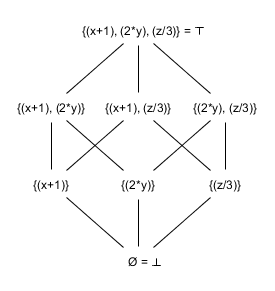
\includegraphics[width=0.5\textwidth]{Hasse}


\section*{Greatest-Lower-Bound:}

\section*{Lattices:}
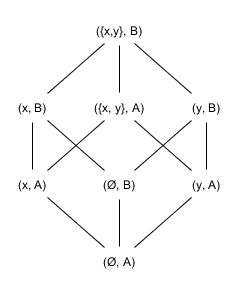
\includegraphics[width=0.5\textwidth]{Lattices}

\noindent A $L_1 \times L_2$ lattice will have $|L_1| * |L_2|$ points. So the resulting lattice will in this case have $2 * 4 = 8$ points.
\section*{Monotone Functions and Fixed-Points:}

\subsection*{i)}
$$X\;=\;\{a,\;b\}$$
$$Y\;=\;X\cup Y$$
In equation form:
$$X\;=\;f(X, Y)\;=\;\{a,\;b\}$$
$$Y\;=\;g(X, Y)\;=\;X\cup Y$$
Can be written as:
$$X\;=\;f()\;=\;\{a,\;b\}$$
$$Y\;=\;g(X, Y)\;=\;X\cup Y$$
The function $f()$ is monotone, as it is constant. Therefore $f() \sqsubseteq f()$ will always hold. The function $g(X,\;Y)$ is also monotone, as no matter which sets use give the function it will combine them and the resulting set will always be greater or equal to the input sets.

\subsection*{ii)}
$$X\;=\;\{a,\;b\}\cup Y$$
$$Y\;=\;X\;\setminus\;\{b\}$$
In equation form:
$$X\;=\;f(X, Y)\;=\;\{a,\;b\}\cup Y$$
$$Y\;=\;g(X, Y)\;=\;X\;\setminus\;\{b\}$$
Can be written as:
$$X\;=\;f(Y)\;=\;\{a,\;b\}\cup Y$$
$$Y\;=\;g(X)\;=\;X\;\setminus\;\{b\}$$
The function $f(Y)$ is monotone, as it return $\{a,\;b\}\cup Y$ which is always a superset of $Y$. The function $g(X)$ is also monotone. It is hard to give an example of why, however intuitively removing a constant element preserves monotonicity, as the same element is removed on both sides of $\sqsubseteq$.
\subsection*{iii)}
$$X\;=\;\{a,\;b\}\cup Z$$
$$Y\;=\;\{a,\;c\}\setminus X$$
$$Z\;=\;X^C$$
In equation form:
$$X\;=\;f(X,\;Y,\;Z)\;=\;\{a,\;b\}\cup Z$$
$$Y\;=\;g(X,\;Y,\;Z)\;=\;\{a,\;c\}\setminus X$$
$$Z\;=\;h(X,\;Y,\;Z)\;=\;X^C$$
Can be written as:
$$X\;=\;f(Z)\;=\;\{a,\;b\}\cup Z$$
$$Y\;=\;g(X)\;=\;\{a,\;c\}\setminus X$$
$$Z\;=\;h(X)\;=\;X^C$$
The function $f(Z)$ is monotone, as it return $\{a,\;b\}\cup Z$ which is always a superset of $Z$. If $g(X)$ is monotone then $\forall\;Y,\;Y'\;P(\{a,\;b,\;c\}):\;Y\;\sqsubseteq\;Y'$. However this is not the case:
$$g(\emptyset)\not\sqsubseteq g(\{a,\;b,\;c\})$$
$$\{a,\;c\}\not\sqsubseteq \emptyset$$
$g(X)$ is therefore not monotone. $h(X)$ is not monotone either, as:
$$g(\emptyset)\not\sqsubseteq g(\{a,\;b,\;c\})$$
$$\{a,\;b\;c\}\not\sqsubseteq \emptyset$$
\end{document}

\subsection*{i)}